\documentclass[final]{article}

\input{poster_style.tex}

% Local layout macros for the paper-flow redesign.
\ifPDFTeX
  \newcommand{\PaperTitleFace}{\sffamily\bfseries}
  \newcommand{\PaperHeaderMetaFace}{\sffamily}
\else
  \IfFileExists{/mnt/c/Windows/Fonts/COPRGTB.TTF}{%
    \newfontfamily\PaperTitleFace[
      Path=/mnt/c/Windows/Fonts/
    ]{COPRGTB.TTF}%
  }{%
    \IfFontExistsTF{Copperplate Gothic Bold}{%
      \newfontfamily\PaperTitleFace{Copperplate Gothic Bold}%
    }{%
      \newcommand{\PaperTitleFace}{\sffamily\bfseries}%
    }%
  }%
  \IfFileExists{/mnt/c/Windows/Fonts/calibri.ttf}{%
    \newfontfamily\PaperHeaderMetaFace[
      Path=/mnt/c/Windows/Fonts/,
      UprightFont=calibri.ttf,
      BoldFont=calibrib.ttf,
      ItalicFont=calibrii.ttf,
      BoldItalicFont=calibriz.ttf
    ]{Calibri}%
  }{%
    \IfFontExistsTF{Calibri}{%
      \newfontfamily\PaperHeaderMetaFace{Calibri}%
    }{%
      \newcommand{\PaperHeaderMetaFace}{\sffamily}%
    }%
  }%
\fi
\renewcommand{\WantedSectionFont}{\PaperHeaderMetaFace\fontsize{27pt}{32pt}\selectfont\bfseries}
\renewcommand{\WantedSubsectionFont}{\PaperHeaderMetaFace\fontsize{20pt}{27pt}\selectfont\bfseries}
\renewcommand{\WantedLabelFont}{\PaperHeaderMetaFace\fontsize{15pt}{20pt}\selectfont\bfseries}

\newcommand{\PaperHeader}[3]{%
  \begin{minipage}[t][74mm][t]{\PosterContentWidth}
    \vspace*{1mm}
    \begin{minipage}[t]{590mm}
      {\PaperTitleFace\fontsize{50pt}{58pt}\selectfont\color{WantedInk}\RaggedRight #1\par}
      \vspace{16mm}
      {\PaperHeaderMetaFace\fontsize{28pt}{34pt}\selectfont\color{WantedText}#2%
        \hspace{4mm}{\fontsize{20pt}{25pt}\selectfont #3}\par}
    \end{minipage}%
    \hfill
    \begin{minipage}[t]{205mm}
      \vspace*{15mm}
      \centering
      \begin{tabular}{@{}c@{\hspace{8mm}}c@{}}
        
\includegraphics[height=54mm,keepaspectratio]{../figures/한양대학교 로고.png}
        &
        
\includegraphics[height=54mm,keepaspectratio]{../figures/통계학회 로고.png}
      \end{tabular}
    \end{minipage}
    \vfill
    {\color{WantedPrimary}\rule{\PosterContentWidth}{2.4mm}}\par
  \end{minipage}
  \vspace{2mm}
}

\newcommand{\PaperSection}[2]{%
  \WantedSectionBar{#1}%
  \vspace{4.8mm}
  {\fontsize{18.8pt}{29pt}\selectfont\color{WantedText}\RaggedRight #2}%
  \vspace{13.5mm}
}

\newcommand{\PaperTinySection}[2]{%
  \WantedSectionBar{#1}%
  \vspace{4mm}
  {\fontsize{18pt}{26.5pt}\selectfont\color{WantedText}\RaggedRight #2}%
  \vspace{7mm}
}

\newcommand{\PaperPlainAbstract}[1]{%
  \vspace*{-7mm}
  \WantedSectionBar{Abstract}%
  \vspace{4.8mm}
  {\fontsize{18.8pt}{29pt}\selectfont\color{WantedText}\RaggedRight #1}%
  \vspace{12mm}
}

\newcommand{\PaperConceptSection}[2]{%
  \WantedSectionBar{#1}%
  \vspace{4.2mm}
  {\fontsize{18.4pt}{27.5pt}\selectfont\color{WantedText}\RaggedRight #2}%
  \vspace{10.5mm}
}

\newcommand{\PaperPlainResultSection}[2]{%
  {\PaperHeaderMetaFace\fontsize{24pt}{30pt}\selectfont\bfseries\color{WantedInk}#1\par}
  \vspace{1.7mm}
  {\color{WantedAccent}\rule{78mm}{0.9mm}}\par
  \vspace{4mm}
  {\fontsize{17.8pt}{26pt}\selectfont\color{WantedText}\RaggedRight #2}%
  \vspace{7mm}
}

\newcommand{\PaperClaim}[1]{%
  {\PaperHeaderMetaFace\fontsize{20.5pt}{27pt}\selectfont\bfseries\color{WantedInk}\RaggedRight #1\par}
  \vspace{3mm}
}

\newcommand{\PaperSubBlockTitle}[1]{%
  \vspace{5mm}
  {\PaperHeaderMetaFace\fontsize{20pt}{25pt}\selectfont\bfseries\color{WantedInk}\RaggedRight #1\par}
  \vspace{1.4mm}
  {\color{WantedAccent}\rule{70mm}{0.85mm}}\par
  \vspace{3mm}
}

\newcommand{\PaperKeyLine}[2]{%
  \begin{minipage}[t]{50mm}
    {\WantedLabelFont\color{WantedAccent}#1}
  \end{minipage}%
  \hspace{4mm}%
  \begin{minipage}[t]{\dimexpr\linewidth-54mm\relax}
    {\fontsize{18.2pt}{26.5pt}\selectfont\color{WantedText}\RaggedRight #2}
  \end{minipage}\par\vspace{3mm}
}

\newcommand{\PaperCompactKeyLine}[2]{%
  \begin{minipage}[t]{34mm}
    {\WantedLabelFont\color{WantedAccent}#1}
  \end{minipage}%
  \hspace{4mm}%
  \begin{minipage}[t]{\dimexpr\linewidth-38mm\relax}
    {\fontsize{16.6pt}{22.5pt}\selectfont\color{WantedText}\RaggedRight #2}
  \end{minipage}\par\vspace{1.3mm}
}

\newcommand{\PaperFailureLine}[2]{%
  \begin{minipage}[t]{62mm}
    {\WantedLabelFont\color{WantedAccent}#1}
  \end{minipage}%
  \hspace{4mm}%
  \begin{minipage}[t]{\dimexpr\linewidth-66mm\relax}
    {\fontsize{17.2pt}{24pt}\selectfont\color{WantedText}\RaggedRight #2}
  \end{minipage}\par\vspace{1.7mm}
}

\newcommand{\PaperBullet}[1]{%
  \begin{minipage}[t]{6mm}
    {\fontsize{18pt}{24pt}\selectfont\color{WantedAccent}\textbullet}
  \end{minipage}%
  \hspace{2mm}%
  \begin{minipage}[t]{\dimexpr\linewidth-8mm\relax}
    {\fontsize{18.2pt}{26.5pt}\selectfont\color{WantedText}\RaggedRight #1}
  \end{minipage}\par\vspace{1.6mm}
}

\newcommand{\PaperQuestionFocus}[1]{%
  \vspace{3mm}
  {\color{WantedPrimary}\rule{\linewidth}{1.1mm}}\par
  \vspace{2.6mm}
  {\PaperHeaderMetaFace\fontsize{15pt}{19pt}\selectfont\bfseries\color{WantedAccent}Key Question\par}
  \vspace{1.6mm}
  {\PaperHeaderMetaFace\fontsize{21pt}{27pt}\selectfont\bfseries\color{WantedInk}\RaggedRight #1\par}
  \vspace{2.8mm}
  {\color{WantedAccent}\rule{0.58\linewidth}{0.8mm}}\par
  \vspace{3.5mm}
}

\newcommand{\PaperReliabilityMetrics}{%
  \vspace{2.8mm}
  {\PaperHeaderMetaFace\fontsize{17pt}{22pt}\selectfont\bfseries\color{WantedInk}Metric definitions\par}
  \vspace{1.6mm}
  \begin{minipage}[t]{0.49\linewidth}
    {\WantedLabelFont\color{WantedAccent}Calibration\par}
    \vspace{0.8mm}
    {\fontsize{12.8pt}{16.5pt}\selectfont
    \[
    \begin{aligned}
    \mathrm{acc}(B)&=\frac{1}{|B|}\sum_{i\in B}\mathbf{1}(\hat y_i=y_i),\\
    \mathrm{conf}(B)&=\frac{1}{|B|}\sum_{i\in B}\max_k p_i(k)
    \end{aligned}
    \]
    \[
    \mathrm{ECE}=\sum_b \frac{|B_b|}{n}\,
    |\mathrm{acc}(B_b)-\mathrm{conf}(B_b)|
    \]}
    {\fontsize{14.2pt}{18.8pt}\selectfont\color{WantedText}\RaggedRight
    ECE summarizes the confidence-accuracy gap across confidence bins.}
  \end{minipage}%
  \hfill
  \begin{minipage}[t]{0.47\linewidth}
    {\WantedLabelFont\color{WantedAccent}OOD ranking\par}
    \vspace{0.8mm}
    {\fontsize{13.8pt}{18pt}\selectfont
    \[
    s(x):\ \text{ID-like score}
    \]
    \[
    \mathrm{AUROC}=P\{s(x_{\mathrm{ID}})>s(x_{\mathrm{OOD}})\}
    \]}
    {\fontsize{14.2pt}{18.8pt}\selectfont\color{WantedText}\RaggedRight
    AUROC summarizes whether ID samples receive higher scores than OOD samples.}
  \end{minipage}\par
}

\newcommand{\PaperResultNote}[2]{%
  \begin{minipage}[t]{28mm}
    {\WantedLabelFont\color{WantedAccent}#1}
  \end{minipage}%
  \hspace{4mm}%
  \begin{minipage}[t]{\dimexpr\linewidth-32mm\relax}
    {\fontsize{16.8pt}{23.5pt}\selectfont\color{WantedText}\RaggedRight #2}
  \end{minipage}\par\vspace{1.4mm}
}

\newcommand{\PaperRightBullet}[1]{%
  \begin{minipage}[t]{5mm}
    {\fontsize{15.6pt}{20.5pt}\selectfont\color{WantedAccent}\textbullet}
  \end{minipage}%
  \hspace{2mm}%
  \begin{minipage}[t]{\dimexpr\linewidth-7mm\relax}
    {\fontsize{15.6pt}{20.5pt}\selectfont\color{WantedText}\RaggedRight #1}
  \end{minipage}\par\vspace{1.35mm}
}

\newlength{\PaperColumnHeight}
\setlength{\PaperColumnHeight}{1040mm}
\setlength{\PosterBodyTopSkip}{4mm}

\newcommand{\PaperTwoColumns}[2]{%
  \vspace*{\PosterBodyTopSkip}
  \begin{minipage}[t][\PaperColumnHeight][t]{\PosterColumnWidth}
    #1
  \end{minipage}%
  \hspace*{\PosterColumnGap}%
  \begin{minipage}[t][\PaperColumnHeight][t]{\PosterColumnWidth}
    #2
  \end{minipage}%
}

\newcommand{\PaperTightTable}[2]{%
  \begingroup
    \fontsize{14.2pt}{19pt}\selectfont
    \color{WantedText}
    \setlength{\tabcolsep}{4.5pt}
    \renewcommand{\arraystretch}{1.18}
    #1
    \par\vspace{2mm}
    {\WantedCaptionFont\color{WantedMuted}#2}
  \endgroup
}

\newcommand{\PaperMicroTable}[2]{%
  \begingroup
    \fontsize{12.2pt}{16.5pt}\selectfont
    \color{WantedText}
    \setlength{\tabcolsep}{2.6pt}
    \renewcommand{\arraystretch}{1.13}
    #1
    \par\vspace{1.6mm}
    {\WantedCaptionFont\color{WantedMuted}#2}
  \endgroup
}

\newcommand{\CalibrationMiniDiagram}{%
  \begin{tikzpicture}[x=13mm,y=13mm]
    \draw[WantedLineStrong, line width=0.55pt] (0,0) -- (4.2,0);
    \draw[WantedLineStrong, line width=0.55pt] (0,0) -- (0,4.1);
    \draw[WantedLine, line width=0.45pt] (0,0) -- (4,4);
    \foreach \x/\h in {0.45/0.35,1.15/0.75,1.85/1.25,2.55/1.85,3.25/2.35} {
      \fill[WantedStatBlue!70] (\x,0) rectangle ++(0.38,\h);
      \draw[WantedStatRed, line width=0.9pt] (\x,{\x+0.35}) -- ++(0.38,0);
    }
    \node[font=\fontsize{7.5pt}{8.5pt}\selectfont, text=WantedMuted] at (2.1,-0.45) {confidence};
    \node[font=\fontsize{7.5pt}{8.5pt}\selectfont, text=WantedMuted, rotate=90] at (-0.5,2.05) {accuracy};
    \node[font=\fontsize{7.5pt}{8.5pt}\selectfont, text=WantedAccent, anchor=west] at (2.5,3.35) {ideal};
    \node[font=\fontsize{7.5pt}{8.5pt}\selectfont, text=WantedStatRed, anchor=west] at (2.5,2.75) {overconfident};
  \end{tikzpicture}%
}

\newcommand{\OODMiniDiagram}{%
  \begin{tikzpicture}[x=12mm,y=12mm]
    \fill[WantedPrimarySoft] (0,0) ellipse (1.35 and 1.0);
    \foreach \x/\y in {-0.9/0.1,-0.5/0.55,-0.35/-0.35,0.15/0.3,0.45/-0.15,0.75/0.45,0.95/-0.45} {
      \fill[WantedStatBlue] (\x,\y) circle (0.075);
    }
    \draw[WantedAccent, line width=0.8pt] (0,0) ellipse (1.35 and 1.0);
    \fill[WantedStatRed] (1.05,0.12) circle (0.12);
    \node[font=\fontsize{7.5pt}{8.5pt}\selectfont, text=WantedStatRed, anchor=west] at (1.2,0.18) {OOD scored ID-like};
    \draw[WantedStatRed, line width=0.6pt, ->] (1.18,0.12) -- (0.98,0.12);
    \node[font=\fontsize{7.5pt}{8.5pt}\selectfont, text=WantedAccent] at (0,-1.25) {ID feature region};
    \node[font=\fontsize{7.5pt}{8.5pt}\selectfont, text=WantedMuted, anchor=west] at (-1.35,1.35) {$s(x)$ should rank ID $>$ OOD};
  \end{tikzpicture}%
}

\newcommand{\EquationLine}[2]{%
  \begin{minipage}[t]{42mm}
    {\WantedLabelFont\color{WantedAccent}#1}
  \end{minipage}%
  \hspace{3mm}%
  \begin{minipage}[t]{\dimexpr\linewidth-45mm\relax}
    {\fontsize{16pt}{22pt}\selectfont #2}
  \end{minipage}\par\vspace{2mm}
}

\newcommand{\OptimizerFeatureOODDiagram}{%
  \vspace{1.5mm}
  \begin{center}
  \resizebox{0.98\linewidth}{!}{%
  \begin{tikzpicture}[x=1mm,y=1mm]
    \node[
      draw=WantedPrimary,
      fill=WantedPrimarySoft,
      rounded corners=3mm,
      line width=0.8pt,
      align=center,
      text width=68mm,
      minimum height=22mm,
      font=\sffamily\bfseries\fontsize{13pt}{16pt}\selectfont
    ] (opt) at (34,0) {Optimizer\\update rule};

    \node[
      draw=WantedAccent,
      fill=white,
      rounded corners=3mm,
      line width=0.8pt,
      align=center,
      text width=82mm,
      minimum height=22mm,
      font=\sffamily\bfseries\fontsize{13pt}{16pt}\selectfont
    ] (dist) at (132,0) {Feature distribution\\$H\mid Y=k:\;(\mu_k,\Sigma_k,\|h\|)$};

    \node[
      draw=WantedPrimary,
      fill=white,
      rounded corners=3mm,
      line width=0.8pt,
      align=center,
      text width=74mm,
      minimum height=22mm,
      font=\sffamily\bfseries\fontsize{13pt}{16pt}\selectfont
    ] (det) at (232,0) {Feature detector\\Maha / kNN / GMM};

    \node[
      draw=WantedStatRed,
      fill=white,
      rounded corners=3mm,
      line width=0.8pt,
      align=center,
      text width=72mm,
      minimum height=22mm,
      font=\sffamily\bfseries\fontsize{13pt}{16pt}\selectfont
    ] (ood) at (326,0) {OOD ranking\\score changes};

    \draw[->, line width=1.2pt, color=WantedPrimary] (opt.east) -- (dist.west);
    \draw[->, line width=1.2pt, color=WantedAccent] (dist.east) -- (det.west);
    \draw[->, line width=1.2pt, color=WantedStatRed] (det.east) -- (ood.west);

    \node[align=center,text=WantedMuted,font=\sffamily\fontsize{10.5pt}{13pt}\selectfont] at (83,-18) {implicit bias};
    \node[align=center,text=WantedMuted,font=\sffamily\fontsize{10.5pt}{13pt}\selectfont] at (181,-18) {detector reads distribution};
    \node[align=center,text=WantedMuted,font=\sffamily\fontsize{10.5pt}{13pt}\selectfont] at (279,-18) {score landscape shifts};
  \end{tikzpicture}}
  \end{center}
  \vspace{1.2mm}
}

\newcommand{\OptimizerMechanismSketch}{%
  \OptimizerFeatureOODDiagram

  \PaperSubBlockTitle{Feature distribution}

  {\fontsize{16.4pt}{21.2pt}\selectfont\color{WantedText}\RaggedRight
  마지막 표현층의 geometry를 class-conditional feature distribution으로 요약한다.
  Let $X$ be an input, $Y\in\{1,\ldots,K\}$ its ID class label, and $H=h_\theta(X)\in\mathbb{R}^p$ the penultimate feature.
  For class $k$, $H\mid Y=k$ is summarized by its center, spread, anisotropy, and norm scale.\par}

  \vspace{0.5mm}
  {\fontsize{16.8pt}{21.5pt}\selectfont
  \[
  H\mid Y=k,\qquad
  \mu_k=\mathbb{E}[H\mid Y=k],\qquad
  \Sigma_k=\mathbb{E}\{(H-\mu_k)(H-\mu_k)^\top\mid Y=k\}.
  \]}
  \vspace{-2mm}
  {\fontsize{14.6pt}{18.8pt}\selectfont\color{WantedText}\RaggedRight
  Here $\mu_k$ is the class center, $\Sigma_k$ describes within-class spread/anisotropy, and $\|H\|_2$ gives the radial feature scale.\par}

  \vspace{-1mm}
  \PaperSubBlockTitle{Feature-based detectors read this distribution}

  \begin{minipage}[t]{0.32\linewidth}
    {\WantedLabelFont\color{WantedAccent}Mahalanobis\par}
    \vspace{-1mm}
    {\fontsize{11.7pt}{14.6pt}\selectfont
    \[
    S_{\mathrm{Maha}}(x)=
    -\min_k (h-\mu_k)^\top
    \Sigma^{-1}(h-\mu_k)
    \]}
    \vspace{-3mm}
    {\fontsize{12.6pt}{15.8pt}\selectfont\color{WantedText}\RaggedRight
    High score: $h$ lies close to some class mean under the pooled covariance ellipsoid.\par}
  \end{minipage}%
  \hfill
  \begin{minipage}[t]{0.30\linewidth}
    {\WantedLabelFont\color{WantedAccent}kNN\par}
    \vspace{-1mm}
    {\fontsize{11.7pt}{14.6pt}\selectfont
    \[
    S_{\mathrm{kNN}}(x)=
    -d_k(h,\mathcal{H}_{\mathrm{ID}})
    \]}
    \vspace{-3mm}
    {\fontsize{12.6pt}{15.8pt}\selectfont\color{WantedText}\RaggedRight
    High score: $h$ has nearby neighbors in the ID feature bank $\mathcal{H}_{\rm ID}$.\par}
  \end{minipage}%
  \hfill
  \begin{minipage}[t]{0.34\linewidth}
    {\WantedLabelFont\color{WantedAccent}DDU-style GMM\par}
    \vspace{-1mm}
    {\fontsize{11.7pt}{14.6pt}\selectfont
    \[
    S_{\mathrm{GMM}}(x)=
    \log\sum_k \pi_k \mathcal{N}(h\mid \mu_k,\Sigma_k)
    \]}
    \vspace{-3mm}
    {\fontsize{12.6pt}{15.8pt}\selectfont\color{WantedText}\RaggedRight
    High score: $h$ has high likelihood under the fitted class-conditional Gaussian mixture.\par}
  \end{minipage}\par

  \vspace{2.4mm}
  {\fontsize{16.2pt}{21pt}\selectfont\color{WantedText}\RaggedRight
  Thus, changing $\mu_k$, $\Sigma_k$, class separation, or feature norm can change the OOD ranking even with the same detector formula.\par}

  \PaperSubBlockTitle{Optimizer mechanism: update rules shape geometry}

  {\fontsize{15.2pt}{19pt}\selectfont
  \[
  z=W h_\theta(x),\quad
  g_t=\nabla_{W_t}L_{\rm CE},\quad
  s_t=W_t^\top\mathbf{1}_K,\quad
  a_t=\frac{1}{K}\|s_t\|_2^2,
  \quad
  g_t^\top\mathbf{1}_K=0.
  \]}
  \vspace{-3mm}
  {\fontsize{13.8pt}{17.4pt}\selectfont\color{WantedText}\RaggedRight
  $s_t$ is the classifier row-sum direction; small $a_t$ means that classifier rows are centered.
  $D_t$ denotes Adam's coordinate-wise adaptive scaling.\par}

  \vspace{2.2mm}
  \begin{minipage}[t]{0.315\linewidth}
    {\color{WantedPrimary}\rule{\linewidth}{0.55mm}}\par
    \vspace{1mm}
    {\PaperHeaderMetaFace\fontsize{14pt}{17pt}\selectfont\bfseries\color{WantedInk}SGD/L2\par}
    \vspace{-2mm}
    {\fontsize{10.9pt}{13.4pt}\selectfont
    \[
    \begin{aligned}
    V_{t+1}&=\beta V_t+g_t,\\
    W_{t+1}&=(1-\eta\lambda)W_t-\eta V_{t+1}.
    \end{aligned}
    \]}
    \vspace{-3mm}
    {\fontsize{12.1pt}{15.1pt}\selectfont\color{WantedText}\RaggedRight
    Because $g_t^\top\mathbf{1}_K=0$, weight decay contracts the row-sum component:\par}
    \vspace{-2mm}
    {\fontsize{10.8pt}{13.2pt}\selectfont
    \[
    s_{t+1}\approx(1-\eta\lambda)s_t.
    \]}
  \end{minipage}%
  \hfill
  \begin{minipage}[t]{0.315\linewidth}
    {\color{WantedAccent}\rule{\linewidth}{0.55mm}}\par
    \vspace{1mm}
    {\PaperHeaderMetaFace\fontsize{14pt}{17pt}\selectfont\bfseries\color{WantedInk}Adam/L2\par}
    \vspace{-2mm}
    {\fontsize{10.9pt}{13.4pt}\selectfont
    \[
    \begin{aligned}
    g_t^{\rm L2}&=g_t+\lambda W_t,\\
    W_{t+1}&=W_t-\eta D_tg_t^{\rm L2}.
    \end{aligned}
    \]}
    \vspace{-3mm}
    {\fontsize{12.1pt}{15.1pt}\selectfont\color{WantedText}\RaggedRight
    The decay term is inside the adaptive direction; in the Adam-like/sign simplification, this can alter the row-sum trajectory toward centering.\par}
  \end{minipage}%
  \hfill
  \begin{minipage}[t]{0.315\linewidth}
    {\color{WantedStatRed}\rule{\linewidth}{0.55mm}}\par
    \vspace{1mm}
    {\PaperHeaderMetaFace\fontsize{14pt}{17pt}\selectfont\bfseries\color{WantedInk}AdamW\par}
    \vspace{-2mm}
    {\fontsize{10.9pt}{13.4pt}\selectfont
    \[
    W_{t+1}=W_t-\eta D_tg_t-\eta\lambda W_t.
    \]
    \[
    (D_tg_t)^\top\mathbf{1}_K\not\equiv0.
    \]}
    \vspace{-4mm}
    {\fontsize{12.1pt}{15.1pt}\selectfont\color{WantedText}\RaggedRight
    Decoupled decay shrinks weights outside the adaptive direction and may not cancel this drift.\par}
  \end{minipage}\par

  \vspace{3mm}
  \PaperKeyLine{Step 1}{CE gradients are row-sum zero, so SGD/L2 mainly contracts the classifier row-sum $s_t$.}
  \PaperKeyLine{Step 2}{Adaptive scaling can turn a centered gradient into a non-centered update; coupled and decoupled weight decay then follow different paths.}
  \PaperKeyLine{Step 3}{NC2/NC3 require classifier rows and centered class means to align, which requires $W^\top\mathbf{1}_K\to0$. Different $s_t$ paths therefore support different class-mean alignment and feature-distribution geometry.}
  \PaperKeyLine{Detector link}{Mahalanobis/kNN/GMM read $\mu_k,\Sigma_k,\|H\|$, and class separation; optimizer-induced geometry changes can therefore change their OOD scores.}
  \PaperKeyLine{Boundary}{This mechanism supports optimizer-induced geometry shifts; OOD reliability is evaluated by the post-hoc diagnostics on the right.}
}

\begin{document}
\begin{WantedPoster}

\PaperHeader
  {Optimizer-Induced Feature Geometry Shapes\\Post-Hoc OOD Detection Reliability}
  {GunHak Jin ∙ HyeYoung Jung}
  {Department of Mathematical Data Science, Hanyang University}

\PaperTwoColumns
{%
  \PaperPlainAbstract{%
    실제 배포환경에서 신뢰성은 단순한 정답률이 아니라 confidence가 실제 정답 가능성과 맞는지, 그리고 학습 분포 밖 입력을 안전하게 거절할 수 있는지까지 포함한다.
    그러나 높은 ID test accuracy는 calibrated confidence나 OOD rejection을 보장하지 않는다.
    본 포스터는 optimizer가 마지막 표현층의 class-conditional feature distribution을 어떻게 바꾸고, Mahalanobis/kNN/GMM 같은 feature-based detector가 그 분포를 읽으면서 OOD score ranking이 어떻게 달라질 수 있는지 진단한다.
    결과적으로 validation-selected high-accuracy model이라도 optimizer/config 선택에 따라 calibration과 feature-based OOD reliability가 달라질 수 있으므로, 배포 전에는 accuracy와 함께 feature distribution-based diagnostics를 확인해야 한다.
  }
  \vspace{2mm}

  \PaperConceptSection{Introduction: Why Accuracy Is Not Reliability}{%
    \PaperClaim{Accuracy is necessary, not reliability.}

    \PaperBullet{ID accuracy는 test distribution에서 정답을 맞춘 비율을 요약한다. 따라서 좋은 모델의 필요조건이지만, 배포환경에서의 신뢰성을 단독으로 보장하지 않는다.}

    \PaperBullet{첫 번째 실패는 miscalibration이다. 모델이 실제 정답 확률보다 더 높은 confidence를 내면, confidence-threshold 기반 승인/보류 결정이 불안정해진다.}

    \PaperBullet{두 번째 실패는 OOD acceptance이다. 학습 분포 밖의 입력이 높은 ID-like score를 받으면, 지원하지 않는 입력도 정상 class prediction으로 downstream decision에 넘어갈 수 있다.}

    \PaperClaim{따라서 신뢰가능한 모델은 높은 accuracy뿐 아니라 calibrated confidence와 OOD input을 구별하는 능력을 함께 가져야 한다.}

    \vspace{2.5mm}
    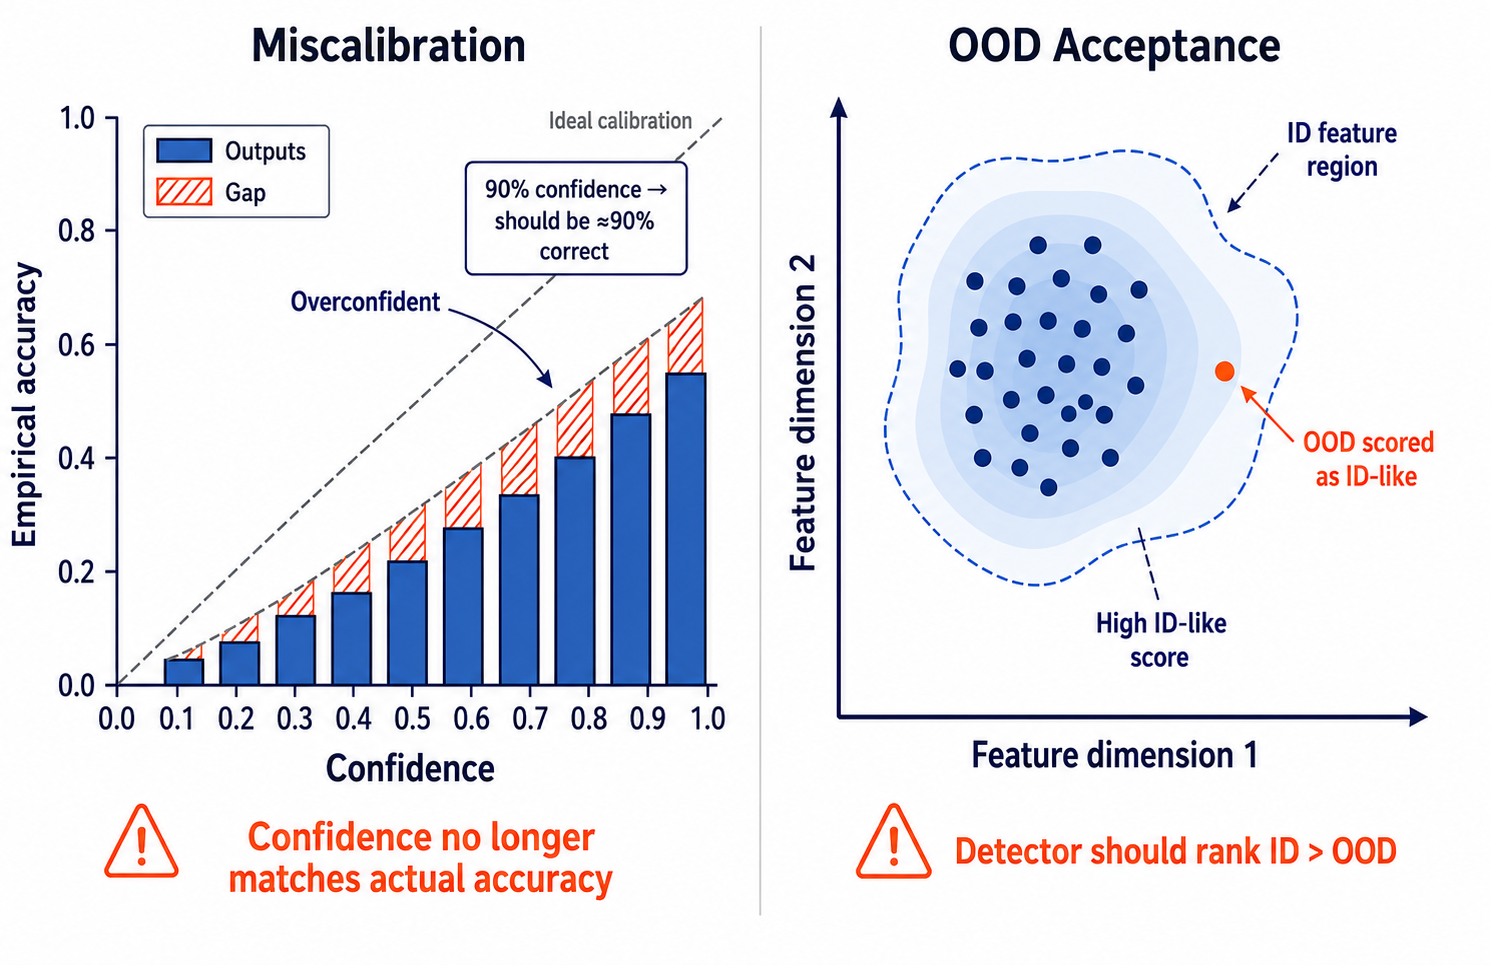
\includegraphics[width=0.97\linewidth]{../figures/final/fig1_reliability_failure_concept.png}\par
    \vspace{1.6mm}
    {\WantedCaptionFont\color{WantedMuted}\RaggedRight
    \textbf{Figure 1.} Accuracy만 높은 모델도 두 방식으로 실패할 수 있다.
    Left: confidence가 empirical accuracy보다 높으면 overconfident decision이 발생한다.
    Right: OOD input이 높은 ID-like score를 받으면 정상 입력처럼 downstream으로 전달될 수 있다.
    Throughout the poster, higher OOD score means more ID-like.\par}

    \PaperSubBlockTitle{Key Question}

    \PaperClaim{최적화 방법이 마지막 표현층의 class-conditional distribution을 다르게 만든다면, validation-selected high-accuracy models의 calibration과 feature-based OOD detection은 어떻게 달라지는가?}

    \PaperFailureLine{Calibration}{ECE는 confidence와 empirical accuracy 사이의 mismatch를 요약한다.}
    \PaperFailureLine{OOD ranking}{AUROC는 ID sample이 OOD sample보다 더 높은 ID-like score를 받는지 평가한다.}
    \PaperFailureLine{This work}{우리는 optimizer name 자체가 아니라, optimizer가 만든 feature distribution과 detector가 읽는 score geometry의 연결을 진단한다.}
  }
  \vspace{8mm}

  \PaperConceptSection{Optimizers: Update Rules Shift Feature Distributions}{%
    \PaperClaim{최적화 방법은 마지막 표현층의 class-conditional feature distribution을 바꿀 수 있다.}
    \OptimizerMechanismSketch
  }
  \vfill

  \PaperConceptSection{Experiment}{%
    \PaperClaim{Selection uses ID validation accuracy only.}
    \begin{minipage}[t]{0.49\linewidth}
      \PaperCompactKeyLine{ID / model}{CIFAR-10 / WRN-28-10}
      \PaperCompactKeyLine{Factors}{SGD, Adam, AdamW over LR-WD grid}
      \PaperCompactKeyLine{Selection}{no OOD/geometry metric used}
    \end{minipage}%
    \hfill
    \begin{minipage}[t]{0.49\linewidth}
      \PaperCompactKeyLine{Post-hoc}{ECE, OOD AUROC, feature geometry metrics}
      \PaperCompactKeyLine{OOD}{CIFAR-100, TinyImageNet, SVHN, MNIST}
      \PaperCompactKeyLine{Reported}{seed 0/1/2 mean $\pm$ sample std}
    \end{minipage}
  }
}
{%
  \PaperTinySection{Figure 2. Accuracy-Matched Reliability Scatter}{%
    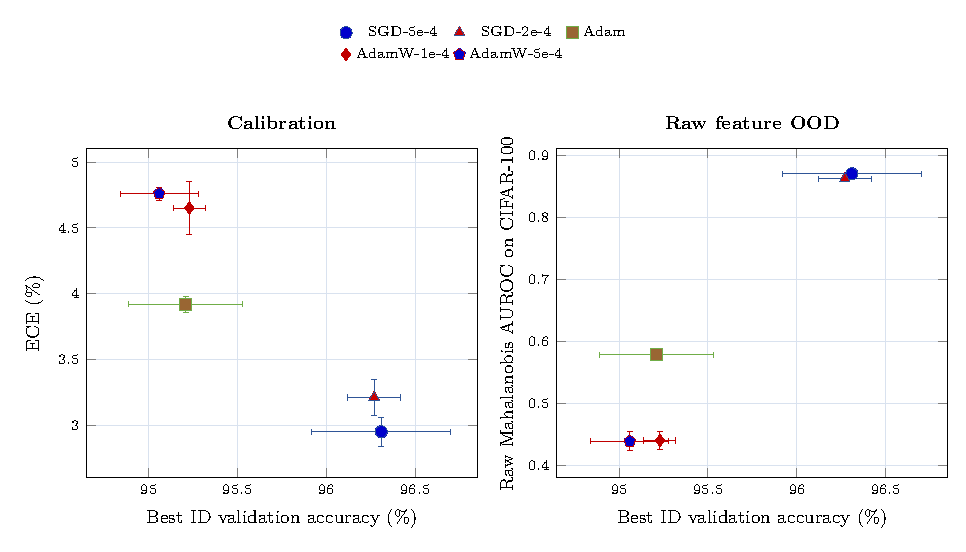
\includegraphics[width=0.99\linewidth]{../figures/final/fig2_wrn350_accuracy_matched_reliability_scatter.pdf}

    \vspace{1mm}
    {\WantedCaptionFont\color{WantedMuted}\RaggedRight
    \textbf{Figure 2.} Points are validation-selected WRN-28-10/CIFAR-10 configs. x-axis is best ID validation accuracy; y-axes show ECE and raw Mahalanobis AUROC on CIFAR-100. Points and error bars are seed0/1/2 mean $\pm$ sample std.\par}

    \vspace{3mm}
    \PaperRightBullet{Similar ID-validation accuracy does not imply identical reliability: ECE and raw feature-OOD AUROC separate by optimizer/config.}
    \PaperRightBullet{SGD points sit at higher validation accuracy with lower ECE; AdamW has Adam-like accuracy but higher ECE and much larger fitted temperature.}
    \PaperRightBullet{This is a post-hoc diagnostic under ID-validation selection; no OOD or geometry metric is used for selection.}
  }

  \PaperTinySection{Figure 3. Raw vs L2 Feature OOD AUROC on Near-OOD}{%
    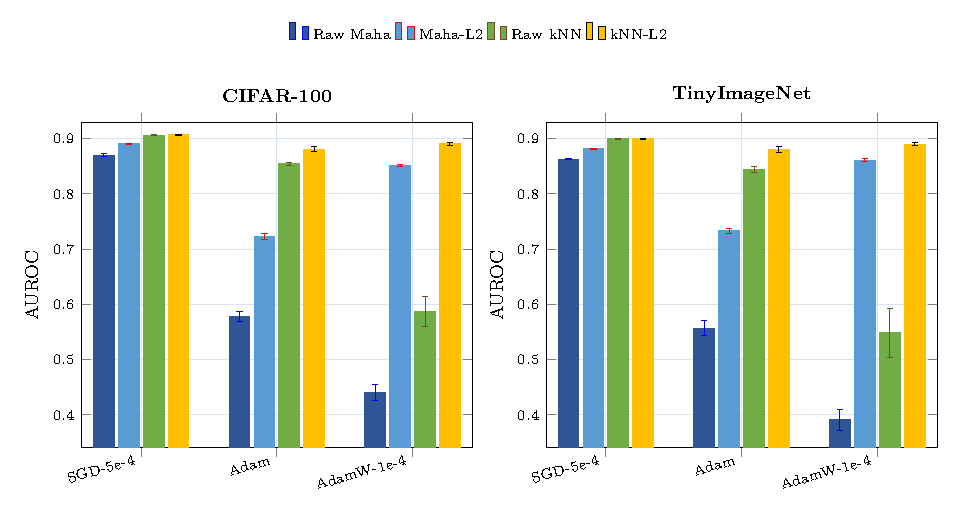
\includegraphics[width=0.99\linewidth]{../figures/final/fig3_wrn350_3optimizer_near_ood_raw_l2.pdf}

    \vspace{1mm}
    {\WantedCaptionFont\color{WantedMuted}\RaggedRight
    \textbf{Figure 3.} One ID-validation representative is shown per optimizer. Bars are AUROC mean $\pm$ sample std over seeds 0/1/2. CIFAR-100 and TinyImageNet are shown separately; higher is better. L2 normalization is a detector-side diagnostic control.\par}

    \vspace{3mm}
    \PaperRightBullet{Raw feature detectors are strongest for the SGD representative and drop for Adam/AdamW, especially under raw Mahalanobis.}
    \PaperRightBullet{L2-normalized controls recover much of the near-OOD ranking for AdamW, indicating a norm/covariance-scale component.}
    \PaperRightBullet{L2 is a diagnostic control, not a final detector solution or full Mahalanobis++ reproduction.}
  }
  \vspace{1mm}

  \PaperTinySection{Table 1. Classwise Covariance Regularization in DDU-Style GMM}{%
    \PaperMicroTable{%
      \begin{tabularx}{\linewidth}{@{}l Z Z Z@{}}
        \toprule
        Optimizer &
        \begin{tabular}[c]{@{}c@{}}gmm\_ddu\_diag\\AUROC\end{tabular} &
        \begin{tabular}[c]{@{}c@{}}gmm\_ddu\_shrinkage\\AUROC\end{tabular} &
        $\Delta$ \\
        \midrule
        SGD & 0.9085 $\pm$ 0.0010 & 0.9103 $\pm$ 0.0010 & +0.0018 \\
        Adam & 0.8678 $\pm$ 0.0027 & 0.8108 $\pm$ 0.0087 & -0.0570 \\
        AdamW & 0.7900 $\pm$ 0.0059 & 0.8112 $\pm$ 0.0051 & +0.0212 \\
        \bottomrule
      \end{tabularx}%
    }{\textbf{Table 1. Classwise covariance regularization in DDU-style GMM (CIFAR-100 AUROC).}
    Representative validation-selected models are shown for SGD, Adam, and AdamW.
    Replacing classwise diagonal covariance with classwise shrinkage covariance slightly improves SGD and clearly improves AdamW, but does not uniformly help every optimizer.
    Results are seed0/1/2 mean $\pm$ sample std.
    This is a DDU-style GMM feature-density diagnostic, not a full DDU reproduction.}

    \vspace{3mm}
    \PaperRightBullet{AdamW shows partial recovery under shrinkage covariance, suggesting that covariance estimation is one part of the detector split.}
    \PaperRightBullet{The effect is not uniform: SGD changes little, while Adam decreases, so shrinkage should be interpreted as a covariance-control diagnostic rather than a universal fix.}
  }

  \PaperTinySection{Table 2. Feature Distribution Geometry}{%
    \PaperMicroTable{%
      \begin{tabularx}{\linewidth}{@{}l l Z Z Z Z@{}}
\toprule
Config & Opt & NC1 $\downarrow$ & InterDist $\uparrow$ & $\|h\|_2$ & Eff. rank \\
\midrule
SGD-5e-4 & SGD & 0.051 $\pm$ 0.002 & 16.62 $\pm$ 0.19 & 14.23 $\pm$ 0.15 & 59.5 $\pm$ 1.8 \\
SGD-2e-4 & SGD & 0.067 $\pm$ 0.002 & 14.28 $\pm$ 0.17 & 12.88 $\pm$ 0.13 & 57.9 $\pm$ 1.1 \\
Adam & Adam & 0.190 $\pm$ 0.002 & 13.34 $\pm$ 0.08 & 14.39 $\pm$ 0.12 & 25.6 $\pm$ 0.4 \\
AdamW-1e-4 & AdamW & 0.277 $\pm$ 0.006 & 5.23 $\pm$ 0.13 & 6.21 $\pm$ 0.09 & 76.9 $\pm$ 6.1 \\
AdamW-5e-4 & AdamW & 0.269 $\pm$ 0.008 & 5.47 $\pm$ 0.07 & 6.50 $\pm$ 0.07 & 74.2 $\pm$ 3.6 \\
\bottomrule
\end{tabularx}
%
    }{ID-train penultimate feature diagnostics, seeds 0/1/2. Lower NC1 and larger InterDist indicate more compact and separated class-conditional geometry. Effective rank is a covariance-spectrum diagnostic, not a causal explanation by itself.}

    \vspace{3mm}
    \PaperRightBullet{The OOD detector split is accompanied by visible geometry shifts in class compactness, separation, norm scale, and covariance spectrum.}
    \PaperRightBullet{AdamW rows have much smaller class-mean separation and lower feature norms than SGD; Adam has larger NC1 than SGD and much lower effective rank.}
    \PaperRightBullet{Distance-, neighbor-, and covariance-based scores can change because the feature distribution they read has changed.}
  }

  \PaperTinySection{Conclusion and Future Work}{%
    {\centering
    {\PaperHeaderMetaFace\fontsize{20.5pt}{27pt}\selectfont\bfseries\color{WantedInk}
    Accuracy-matched models are not reliability-matched: feature geometry determines post-hoc detector behavior.\par}
    }
    \vspace{3mm}

    {\fontsize{15.6pt}{20.5pt}\selectfont\color{WantedText}\RaggedRight
    Across validation-selected WRN-28-10/CIFAR-10 configurations, similar ID validation accuracy does not imply similar calibration or feature-based OOD reliability.
    The observed split is accompanied by changes in penultimate class-conditional geometry, including compactness, class separation, feature-norm scale, and covariance structure.
    Detector-side controls such as L2 normalization and shrinkage covariance explain part of the gap, but their effects are not uniform; therefore, they should be treated as diagnostics rather than universal fixes.
    These results support a practical conclusion: deployment-oriented model selection should jointly inspect accuracy, calibration, OOD ranking, and feature-distribution geometry.\par}

    \vspace{2.5mm}
    \PaperRightBullet{\textbf{Broader architectures and datasets.} Extend the study beyond WRN-28-10/CIFAR-10 to more diverse architectures and training datasets.}
    \PaperRightBullet{\textbf{Other training interventions.} Test whether other optimization methods, such as SAM, and augmentation strategies, such as mixup, preserve or distort detector-relevant feature geometry.}
    \PaperRightBullet{\textbf{Mechanistic analysis.} Clarify how representation-layer distribution changes propagate to the output layer and affect generalization and ECE.}
  }
}

\WantedFooter
  {WRN-28-10/CIFAR-10 selected configs, seeds 0/1/2. OOD and geometry metrics are post-hoc diagnostics; higher OOD score means more ID-like.}
  {Source: poster/poster.tex; DDU-style GMM feature density is diagnostic, not a full DDU reproduction.}

\end{WantedPoster}
\end{document}
